% ============================================================
% pipeline_flow.tex — One-Time Visual: Vol-Arb Project Flow
% ============================================================
% Compile: pdflatex pipeline_flow.tex
% Standalone diagram showing data flow, scripts, and outputs.
% ============================================================

\documentclass[11pt,landscape,a4paper]{standalone}
\usepackage[margin=0.6in]{geometry}
\usepackage{tikz}
\usepackage{amsmath}
\usetikzlibrary{
    shapes.geometric,
    arrows.meta,
    positioning,
    fit,
    backgrounds,
    calc,
    decorations.pathreplacing
}

% Refined color palette
\definecolor{inputfill}{HTML}{E3F2FD}
\definecolor{stagefill}{HTML}{E8F5E9}
\definecolor{scriptfill}{HTML}{FFF3E0}
\definecolor{outputfill}{HTML}{F3E5F5}
\definecolor{modulefill}{HTML}{FAFAFA}

\tikzset{
    input/.style={
        rectangle, draw=blue!60, fill=inputfill,
        rounded corners=3pt, line width=0.6pt,
        minimum width=2cm, minimum height=0.55cm,
        font=\small\bfseries
    },
    stage/.style={
        rectangle, draw=green!50!black!60, fill=stagefill,
        rounded corners=3pt, line width=0.6pt,
        minimum width=2.2cm, minimum height=0.55cm,
        font=\small\bfseries
    },
    script/.style={
        rectangle, draw=orange!70!black!50, fill=scriptfill,
        rounded corners=3pt, line width=0.5pt,
        minimum width=1.9cm, minimum height=0.5cm,
        font=\footnotesize
    },
    output/.style={
        rectangle, draw=purple!60, fill=outputfill,
        rounded corners=3pt, line width=0.5pt,
        minimum width=1.7cm, minimum height=0.45cm,
        font=\footnotesize
    },
    module/.style={
        rectangle, draw=gray!40, fill=modulefill,
        rounded corners=2pt, line width=0.4pt,
        minimum width=1.6cm, minimum height=0.4cm,
        font=\scriptsize\ttfamily
    },
    arrow/.style={-{Stealth[length=2.2mm]}, line width=0.8pt, draw=gray!70},
    thinarrow/.style={-{Stealth[length=1.8mm]}, line width=0.5pt, draw=gray!60},
    sectionlabel/.style={font=\scriptsize\sffamily\bfseries, text=gray!70}
}

\begin{document}
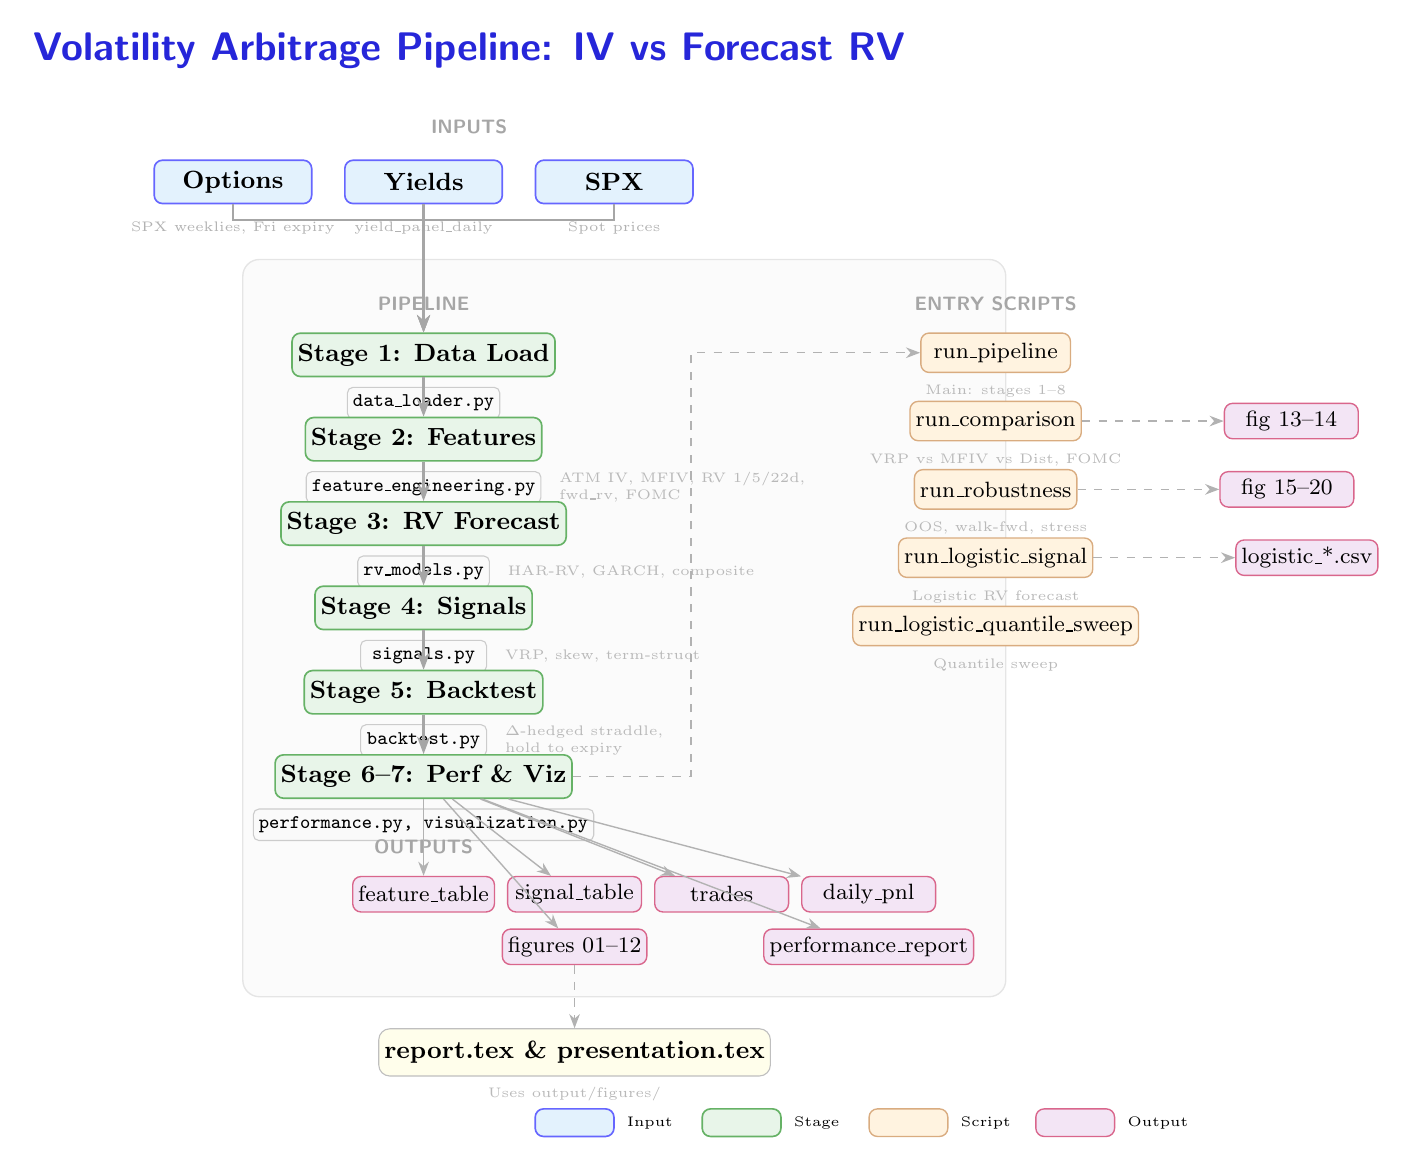
\begin{tikzpicture}[
    node distance=0.4cm and 0.6cm,
    every node/.style={inner sep=2pt}
]

% ═══════════════════════════════════════════════════════════
%  TITLE
% ═══════════════════════════════════════════════════════════
\node[font=\Large\bfseries\sffamily, text=gray!30!blue] (title)
    {Volatility Arbitrage Pipeline: IV vs Forecast RV};

% ═══════════════════════════════════════════════════════════
%  INPUT DATA
% ═══════════════════════════════════════════════════════════
\node[sectionlabel, below=0.5 of title] (inlabel) {INPUTS};

\node[input, below=0.25 of inlabel, xshift=-3cm] (opt) {Options};
\node[input, right=0.4 of opt] (yld) {Yields};
\node[input, right=0.4 of yld] (spx) {SPX};

\node[below=0.15 of opt, font=\tiny, text=gray!60] (optd) {SPX weeklies, Fri expiry};
\node[below=0.15 of yld, font=\tiny, text=gray!60] (yldd) {yield\_panel\_daily};
\node[below=0.15 of spx, font=\tiny, text=gray!60] (spxd) {Spot prices};

% ═══════════════════════════════════════════════════════════
%  MAIN PIPELINE (vertical flow)
% ═══════════════════════════════════════════════════════════
\node[sectionlabel, below=1.1 of yld] (plabel) {PIPELINE};

\node[stage, below=0.2 of plabel] (load) {Stage 1: Data Load};
\node[module, below=0.12 of load] (dl) {data\_loader.py};

\draw[arrow] (opt.south) -- ++(0,-0.2) -| (load.north);
\draw[arrow] (yld) -- (load);
\draw[arrow] (spx.south) -- ++(0,-0.2) -| (load.north);

\node[stage, below=0.5 of load] (feat) {Stage 2: Features};
\node[module, below=0.12 of feat] (fe) {feature\_engineering.py};
\node[right=0.15 of fe, font=\tiny, text=gray!55, align=left] (felist) {ATM IV, MFIV, RV 1/5/22d,\\fwd\_rv, FOMC};
\draw[arrow] (load) -- (feat);

\node[stage, below=0.5 of feat] (rv) {Stage 3: RV Forecast};
\node[module, below=0.12 of rv] (rvm) {rv\_models.py};
\node[right=0.15 of rvm, font=\tiny, text=gray!55] (rvlist) {HAR-RV, GARCH, composite};
\draw[arrow] (feat) -- (rv);

\node[stage, below=0.5 of rv] (sig) {Stage 4: Signals};
\node[module, below=0.12 of sig] (sigm) {signals.py};
\node[right=0.15 of sigm, font=\tiny, text=gray!55] (siglist) {VRP, skew, term-struct};
\draw[arrow] (rv) -- (sig);

\node[stage, below=0.5 of sig] (bt) {Stage 5: Backtest};
\node[module, below=0.12 of bt] (btm) {backtest.py};
\node[right=0.15 of btm, font=\tiny, text=gray!55, align=left] (btlist) {$\Delta$-hedged straddle,\\hold to expiry};
\draw[arrow] (sig) -- (bt);

\node[stage, below=0.5 of bt] (perf) {Stage 6--7: Perf \& Viz};
\node[module, below=0.12 of perf] (perfm) {performance.py, visualization.py};
\draw[arrow] (bt) -- (perf);

% ═══════════════════════════════════════════════════════════
%  OUTPUTS
% ═══════════════════════════════════════════════════════════
\node[sectionlabel, below=0.45 of perf] (outlabel) {OUTPUTS};

\node[output, below=0.2 of outlabel] (out1) {feature\_table};
\node[output, right=0.15 of out1] (out2) {signal\_table};
\node[output, right=0.15 of out2] (out3) {trades};
\node[output, right=0.15 of out3] (out4) {daily\_pnl};
\node[output, below=0.2 of out2] (out5) {figures 01--12};
\node[output, below=0.2 of out4] (out6) {performance\_report};

\draw[thinarrow] (perf) -- (out1);
\draw[thinarrow] (perf) -- (out2);
\draw[thinarrow] (perf) -- (out3);
\draw[thinarrow] (perf) -- (out4);
\draw[thinarrow] (perf) -- (out5);
\draw[thinarrow] (perf) -- (out6);

% ═══════════════════════════════════════════════════════════
%  ENTRY SCRIPTS (right panel)
% ═══════════════════════════════════════════════════════════
\node[sectionlabel, right=5.5 of plabel] (sclabel) {ENTRY SCRIPTS};

\node[script, below=0.2 of sclabel] (rp) {run\_pipeline};
\node[below=0.08 of rp, font=\tiny, text=gray!55] (rpd) {Main: stages 1--8};

\node[script, below=0.35 of rp] (rc) {run\_comparison};
\node[below=0.08 of rc, font=\tiny, text=gray!55] (rcd) {VRP vs MFIV vs Dist, FOMC};

\node[script, below=0.35 of rc] (rr) {run\_robustness};
\node[below=0.08 of rr, font=\tiny, text=gray!55] (rrd) {OOS, walk-fwd, stress};

\node[script, below=0.35 of rr] (rls) {run\_logistic\_signal};
\node[below=0.08 of rls, font=\tiny, text=gray!55] (rlsd) {Logistic RV forecast};

\node[script, below=0.35 of rls] (rlq) {run\_logistic\_quantile\_sweep};
\node[below=0.08 of rlq, font=\tiny, text=gray!55] (rlqd) {Quantile sweep};

% Script outputs
\node[output, right=1.8 of rc] (cmp1) {fig 13--14};
\node[output, right=1.8 of rr] (rob1) {fig 15--20};
\node[output, right=1.8 of rls] (log1) {logistic\_*.csv};

\draw[thinarrow, dashed] (perf.east) -- ++(1.5,0) |- (rp.west);
\draw[thinarrow, dashed] (rc) -- (cmp1);
\draw[thinarrow, dashed] (rr) -- (rob1);
\draw[thinarrow, dashed] (rls) -- (log1);

% ═══════════════════════════════════════════════════════════
%  REPORT
% ═══════════════════════════════════════════════════════════
\node[
    draw=gray!50, fill=yellow!8, rounded corners=4pt,
    minimum width=4.5cm, minimum height=0.6cm,
    font=\small\bfseries, below=0.8 of out5
] (report) {report.tex \& presentation.tex};
\node[below=0.06 of report, font=\tiny, text=gray!55] (repd)
    {Uses output/figures/};

\draw[thinarrow, dashed] (out5.south) -- ++(0,-0.25) -| (report.north);

% ═══════════════════════════════════════════════════════════
%  LEGEND
% ═══════════════════════════════════════════════════════════
\node[input, below=0.4 of report, minimum width=1cm, minimum height=0.35cm] (l1) {};
\node[right=0.08 of l1, font=\tiny, anchor=west] {Input};
\node[stage, right=1.1 of l1, minimum width=1cm, minimum height=0.35cm] (l2) {};
\node[right=0.08 of l2, font=\tiny, anchor=west] {Stage};
\node[script, right=1.1 of l2, minimum width=1cm, minimum height=0.35cm] (l3) {};
\node[right=0.08 of l3, font=\tiny, anchor=west] {Script};
\node[output, right=1.1 of l3, minimum width=1cm, minimum height=0.35cm] (l4) {};
\node[right=0.08 of l4, font=\tiny, anchor=west] {Output};

% ═══════════════════════════════════════════════════════════
%  BACKGROUND: subtle pipeline box
% ═══════════════════════════════════════════════════════════
\begin{scope}[on background layer]
    \node[fit=(plabel)(load)(feat)(rv)(sig)(bt)(perf)(outlabel)(out1)(out2)(out3)(out4)(out5)(out6),
        rounded corners=6pt, fill=gray!3, draw=gray!20, line width=0.5pt,
        inner sep=0.4cm] (pipelinebox) {};
\end{scope}

\end{tikzpicture}
\end{document}
